%%%%%%%%%%%%%%%%%%%%%%%%%%%%%%%%%%%%%%%%%%%%%%%%%%%%%%%%%%%%%%%%%%%%%%%%%%%%%%%%
%%%%%%%%%%%%%%%%%%   Vorlage für eine Abschlussarbeit   %%%%%%%%%%%%%%%%%%%%%%%%
%%%%%%%%%%%%%%%%%%%%%%%%%%%%%%%%%%%%%%%%%%%%%%%%%%%%%%%%%%%%%%%%%%%%%%%%%%%%%%%%

% Erstellt von Maximilian Nöthe, <maximilian.noethe@tu-dortmund.de>
% ausgelegt für lualatex und Biblatex mit biber

% Kompilieren mit
% latexmk --lualatex --output-directory=build thesis.tex
% oder einfach mit:
% make

\documentclass[
  tucolor,       % remove for less green,
  parskip=full,  % new paragraphs start with half line vertical space
  open=any,      % chapters start on both odd and even pages
  cleardoublepage=plain,  % no header/footer on blank pages
]{tudothesis}

\setlength{\parindent}{0pt}


% Warning, if another latex run is needed
\usepackage[aux]{rerunfilecheck}

% just list chapters and sections in the toc, not subsections or smaller
\setcounter{tocdepth}{3}

%------------------------------------------------------------------------------
%------------------------------ Fonts, Unicode, Language ----------------------
%------------------------------------------------------------------------------
\usepackage{fontspec}
\defaultfontfeatures{Ligatures=TeX}  % -- becomes en-dash etc.

% load english (for abstract) and ngerman language
% the main language has to come last
% Use line below if thesis is written in german
% \usepackage[american, ngerman]{babel}
% Use line below if thesis is written in english
\usepackage[ngerman, american]{babel}

% intelligent quotation marks, language and nesting sensitive
\usepackage[autostyle]{csquotes}

% microtypographical features, makes the text look nicer on the small scale
\usepackage{microtype}

%------------------------------------------------------------------------------
%------------------------ Math Packages and settings --------------------------
%------------------------------------------------------------------------------

\usepackage{amsmath}
\usepackage{amssymb}
\usepackage{mathtools}

% Enable Unicode-Math and follow the ISO-Standards for typesetting math
\usepackage[
  math-style=ISO,
  bold-style=ISO,
  sans-style=italic,
  nabla=upright,
  partial=upright,
  warnings-off={mathtools-colon,mathtools-overbracket}, % suppress some unnecessary warnings
]{unicode-math}
\setmathfont{Latin Modern Math}

% nice, small fracs for the text with \sfrac{}{}
\usepackage{xfrac}


%------------------------------------------------------------------------------
%---------------------------- Numbers and Units -------------------------------
%------------------------------------------------------------------------------

\usepackage[
  locale=DE,
  separate-uncertainty=true,
  per-mode=symbol-or-fraction,
]{siunitx}

\addto\extrasngerman{\sisetup{locale = DE}}
\addto\extrasenglish{\sisetup{locale = US}}

%------------------------------------------------------------------------------
%-------------------------------- tables  -------------------------------------
%------------------------------------------------------------------------------

\usepackage{booktabs}       % \toprule, \midrule, \bottomrule, etc

%------------------------------------------------------------------------------
%-------------------------------- graphics -------------------------------------
%------------------------------------------------------------------------------

\usepackage{graphicx}
% currently broken
% \usepackage{grffile}

% allow figures to be placed in the running text by default:
\usepackage{scrhack}
\usepackage{float}
\floatplacement{figure}{htbp}
\floatplacement{table}{htbp}

% keep figures and tables in the section
\usepackage[section, below]{placeins}

% allows to include PDFs as full pages
\usepackage{pdfpages}

% Set the PDF Version of this document to 1.7 (1.4 is the current default)
% This is needed so that PDFs with Version >1.5 can be included
\pdfvariable minorversion=7

%------------------------------------------------------------------------------
%---------------------- customize list environments ---------------------------
%------------------------------------------------------------------------------

\usepackage{enumitem}

%------------------------------------------------------------------------------
%------------------------------ Bibliographie ---------------------------------
%------------------------------------------------------------------------------

\usepackage[
  backend=biber,   % use modern biber backend
  autolang=hyphen, % load hyphenation rules for if language of bibentry is not
                   % german, has to be loaded with \setotherlanguages
                   % in the references.bib use langid={en} for english sources
]{biblatex}
\addbibresource{references.bib}  % the bib file to use
\DefineBibliographyStrings{german}{andothers = {{et\,al\adddot}}}  % replace u.a. with et al.


% Last packages, do not change order or insert new packages after these ones
\usepackage[pdfusetitle, unicode, linkbordercolor=tugreen, citebordercolor=tugreen]{hyperref}
\usepackage{bookmark}
\usepackage[shortcuts]{extdash}

%------------------------------------------------------------------------------
%-------------------------    Angaben zur Arbeit   ----------------------------
%------------------------------------------------------------------------------

\author{Akram Aki}
\title{CINIC-10 Source Classifier: Learning to Tell CIFAR from ImageNet}
\date{2025}
\birthplace{Hagen, Germany}
\chair{WG Rhode / Elsässer}
\division{Fakultät Physik}
\thesisclass{Machine Learning for Physicists}
\submissiondate{31. August 2025}
\firstcorrector{Dr.~Carsten~Burgard}
\secondcorrector{Dr.~Cornelius~Grunwald}

% tu logo on top of the titlepage
\titlehead{
\includegraphics[height=1.5cm]{logos/tu-logo.pdf}}

\begin{document}
%\frontmatter
\maketitle

% Gutachterseite
\makecorrectorpage

% hier beginnt der Vorspann, nummeriert in römischen Zahlen
\thispagestyle{plain}

\section*{Abstract}
The goal of this project was to build a classifier capable of determining whether an image in the CINIC-10 dataset originates from CIFAR-10 or from ImageNet. 
To this end, we analyzed statistical and visual differences between the two domains, including RGB mean values, per-class variance and structural image characteristics.
We tested various machine learning approaches, including Convolutional Neural Networks (CNNs), Multi-Layer Perceptrons (MLPs) as well as classical models like Random Forests. 
In addition to training models, we explored interpretability techniques such as visualizing activation maps and analyzing learned convolutional filters. 
The results show that even without class labels, models can learn to distinguish the source domain of images based on subtle differences in data characteristics.
All code and instructions to reproduce the results are available in the associated GitHub repository~\cite{cinic10-source-classifier}.

\section*{Kurzfassung}
\begin{foreignlanguage}{german}
In diesem Projekt wurde das Ziel verfolgt, einen Klassifikator zu entwickeln, der innerhalb des CINIC-10-Datensatzes erkennen kann, ob ein Bild ursprünglich aus CIFAR-10 oder aus ImageNet 
stammt. Dafür wurden zunächst die Metadaten ausgewertet und visuelle sowie statistische Unterschiede zwischen den beiden Quellen analysiert, z.B. RGB-Mittelwerte, 
Varianz pro Klasse und Strukturmerkmale der Bilder.
Zur Modellentwicklung wurden verschiedene Machine Learning Ansätze getestet, darunter Convolutional Neural Networks (CNNs), Multi-Layer Perceptrons (MLPs) sowie klassische Verfahren wie 
Random Forests.
Neben der Modellierung wurden auch Ansätze zur Interpretation der Modelle verfolgt, etwa durch Visualisierung einzelner Bilder nach durchlauf des Kernel Filters oder 
durch die Visualisierung gelernter Filter. 
Das Projekt zeigt, dass auch ohne explizite Objektklassenunterscheidung Unterschiede in der Datenquelle durch maschinelles Lernen erkannt werden können.
Der vollständige Code sowie eine Anleitung für Basis Einstellungen sind im zugehörigen GitHub-Repository~\cite{cinic10-source-classifier} zu finden.
\end{foreignlanguage}

\newpage 
\tableofcontents

\newpage

%\mainmatter
% Hier beginnt der Inhalt mit Seite 1 in arabischen Ziffern
\section{Introduction}

The automated classification of visual data is one of the central tasks in modern machine learning. Over the past decade, datasets such as \textbf{CIFAR-10} and \textbf{ImageNet} have played a 
pivotal role in the development and evaluation of deep learning models. These datasets differ not only in resolution and content diversity, but also in how images are collected, 
preprocessed, and labeled. While CIFAR-10 consists of small, uniformly processed images of objects centered against clean backgrounds, ImageNet offers a broader and more varied selection 
of real world scenes.
The \textbf{CINIC-10 dataset} (CINIC = \textit{CINIC Is Not ImageNet or CIFAR}) merges images from CIFAR-10 and downsampled ImageNet into a unified 10-class structure. 
It was primarily created to bridge the gap between the simplicity of CIFAR-10 and the complexity of ImageNet, enabling more robust benchmarking. However, this fusion may also 
introduce domain-specific artifacts, which could prevent certain machine learning approaches from reaching their full potential.
In this project, we explore the question:
\begin{center}
\textbf{\textit{Can a ML model distinguish the original source of an image in CINIC-10?}}
\end{center}
To answer this, we analyzed the dataset at multiple levels. First, we investigated low-level statistical properties, such as per-class RGB channel means and variances, to detect structural 
biases between the two sources. For instance, CIFAR-10 images often appear more ``stock-like'', meaning well-centered, consistently lit, and visually uniform. ImageNet derived images tend 
to be more diverse, naturalistic, and less curated in appearance.
Second, we trained a variety of models, ranging from shallow multi-layer perceptrons to convolutional neural networks (CNNs), to predict the image source. 
We also experimented with classical machine learning methods such as random forests and compared their performance to neural models. 
Custom data generators were implemented to efficiently stream image batches during training, allowing us to scale to tens of thousands of samples without exceeding memory limits.
In addition to evaluating model performance, we investigated interpretability. We visualized feature maps and learned convolutional kernels to better understand how the models identify 
domain specific features and whether these features reflect meaningful differences between CIFAR-10 and ImageNet samples.
This report presents the dataset and the formulation of the source classification task, outlines the modeling approaches and discusses our findings with a 
focus on accuracy and what the models may have learned about image domain differences.

While this report assumes basic familiarity with machine learning, no deep technical expertise is required to follow the main arguments. Readers unfamiliar with core concepts such 
as neural networks, convolutional layers, or decision trees may refer to the external resources listed in Appendix~\ref{sec:further-reading}. 
These sources provide brief and accessible introductions to the most important topics mentioned throughout the report.
\section{Background and Related Work}

Image classification is a foundational task in computer vision and has been extensively studied through standardized benchmark datasets such as \textbf{CIFAR-10} 
\cite{krizhevsky2009learning} and \textbf{ImageNet} \cite{deng2009imagenet}. CIFAR-10 consists of low-resolution (32x32) images across 10 object categories, 
designed for rapid prototyping of deep learning models. In contrast, ImageNet offers millions of high-resolution, hierarchically organized images, capturing a wide variety of real-world content.

The \textbf{CINIC-10} dataset \cite{darlow2018cinic} was introduced to bridge the gap between CIFAR-10 and ImageNet in both scale and diversity. It consists of 
270,000 32x32 RGB images equally distributed across the same 10 classes as CIFAR-10. 60,000 datapoints originate from CIFAR-10, and the other 210,000 comprises downsampled ImageNet 
images mapped to equivalent CIFAR-10 categories. While CINIC-10 was primarily designed for benchmarking and training stability evaluation, the inclusion of two distinct data sources 
introduces an implicit domain shift within each class.

\textbf{Domain shift}, the phenomenon where data distributions differ between training and testing environments, has been extensively studied in the contexts of domain adaptation and 
generalization \cite{wang2018deep}. Prior work has shown that even subtle differences in image statistics, such as background texture, object positioning, or lighting, can significantly 
affect model performance and generalizability \cite{torralba2011unbiased, recht2019imagenet}. These differences are often referred to as dataset bias, and models may learn to exploit such 
artifacts rather than focusing on semantically meaningful content.

The presence of label noise is another important consideration when working with large-scale datasets. Northcutt et al. \cite{northcutt2021confident} identified that datasets like ImageNet 
may contain a non-trivial amount of mislabeled images, potentially impacting training dynamics and evaluation reliability.

Our work builds on these observations by explicitly formulating a \textit{source classification} task within CINIC-10. Instead of predicting object classes, we focus on whether a model
can identify whether an image originated from CIFAR-10 or ImageNet. To our knowledge, this direction—treating source domain as a predictive label—has received relatively little attention. 
The only closely related work we are aware of is the "Guess the Dataset" experiment proposed by Torralba and Efros in their paper \textit{Unbiased Look at Dataset Bias} 
\cite{torralba2011unbiased}, where human participants were asked to classify the dataset origin of an image. 
Their work emphasizes how visual characteristics unrelated to semantic content, such as lighting, resolution, and framing, can allow both humans and models to identify dataset membership, 
highlighting the presence of strong, exploitable dataset specific artifacts.

\chapter{Struktur der Arbeit}

Eine mögliche Struktur der Arbeit sieht wie folgt aus:

\begin{enumerate}
    \item \textbf{Einleitung}\\
        In der \emph{kurzen} Einleitung wird die Motivation für die Arbeit
        dargestellt und ein Einblick in die kommenden Kapitel gegeben.
    \item \textbf{Theoretische Grundlagen}\\
        Alles was an theoretischen Grundlagen benötigt wird, sollte auch eher kurz gehalten werden.
        Statt Grundlagenwissen zu präsentieren, eher auf die entsprechenden Lehrbücher verweisen.
        Etwa: Tiefer gehende Informationen zur klassischen Mechanik entnehmen Sie bitte \cite{kuypers}.
    \item \textbf{Ergebnisse} \\
        Der eigentliche Teil der Arbeit, das was getan wurde.
    \item \textbf{Zusammenfassung und Ausblick} \\
        Zusammenfassung der Ergebnisse, Optimierungsmöglichkeiten, mögliche weitergehende Untersuchungen.
\end{enumerate}

Die Gliederung sollte auf der einen Seite nicht zu fein sein, auf der anderen Seite
sollten sich klar unterscheidende Abschnitte auch kenntlich gemacht werden.

In der hier verwendeten \KOMAScript-Klasse \texttt{scrbook} ist die oberste Gliederungsebene,
die in der Bachelorarbeit verwendet werden sollte, das \texttt{\textbackslash chapter}.

Ein Kapitel sollte erst dann in tiefere Gliederungsebenen unterteilt werden, wenn es auch wirklich etwas zu unterteilen gibt. Es sollte keine Kapitel mit nur einem Unterkapitel (\texttt{\textbackslash section}) geben.

In dieser Vorlage ist die Tiefe des Inhaltsverzeichnisses auf \texttt{chapter} und \texttt{section} beschränkt. Möchten Sie diese Beschränkung aufheben, entfernen Sie den Befehl
\begin{verbatim}
            \setcounter{tocdepth}{1}
\end{verbatim}
aus der Präambel oder ändern Sie den Zahlenwert entsprechend. Das Inhaltsverzeichnis sollte für eine Bachelorarbeit auf eine Seite passen.

\section{Wichtige Hinweise zum Dokument}\label{make}

Diese Vorlage ist auf die Kompilierung mit \texttt{lualatex} ausgelegt. 
Als Dokumentenklasse  wird die \KOMAScript\-Klasse \texttt{scrbook} verwendet.
Falls Sie Änderungen am Layout vornehmen möchten, lesen Sie die \KOMAScript-Dokumentation: \cite{koma}.

Eine umfangreiche Einführung in die moderne Verwendung von \LaTeX{} gibt es hier: \cite{toolbox}, lesenswert ist außerdem das \LaTeX-Tabu: \cite{l2tabu}

Um dieses Dokument vollständig zu erstellen sind maximal vier Programmläufe nötig:
\begin{enumerate}[nosep]
    \item \texttt{lualatex BachelorArbeit.tex}
    \item \texttt{biber BachelorArbeit.bcf}
    \item \texttt{lualatex BachelorArbeit.tex}
    \item \texttt{lualatex BachelorArbeit.tex}
\end{enumerate}

Beim ersten Lauf des \LaTeX-Compilers werden die Kapitel, Links und zitierten Bibliographieeinträge in Hilfsdateien geschrieben.

Dann ist ein Lauf des Programms \texttt{biber} nötig, welches die benötigten Einträge aus der Hilfsdatei einliest, die Einträge aus der \texttt{.bib} Datei einliest, sortiert und formatiert und in eine weitere Hilfsdatei schreibt.

Beim nächsten \LaTeX-Lauf werden dann diese Hilfsdateien eingelesen und Literatur- und Inhaltsverzeichnis erstellt.

Manchmal ist ein vierter Lauf nötig, falls sich durch das einfügen des Literaturverzeichnisses Seitenzahlen verändert haben.

Das Tool \texttt{latexmk} übernimmt dies mit nur einem Programmaufruf und
führ nur so viele Aufrufe durch, wie nötig sind.

\texttt{latexmk --lualatex BachelorArbeit.tex}

Eine gute Option ist es, den \LaTeX{} Output in einem anderen 
Ordner zu erzeugen, dies ist mit der \texttt{--output-directory} Option möglich:

\texttt{latexmk --output-directory=build --lualatex BachelorArbeit.tex}


\subsection{Erstellen des Ausgabedokuments mit Make}

Für diese Vorlage wird ein Makefile zur Verfügung gestellt, welches automatisch alle Schritte ausführt, die für das fertige Dokument nötig sind.
Die Ausgabe erfolgt dabei in den Unterordner \texttt{build/}.
Make prüft, ob die Quelldateien verändert wurden, falls nicht, werden auch keine Befehle ausgeführt.

Falls Sie das Makefile benutzen möchten, sollten Sie alle Abhängigkeiten eintragen (Eigene Dateien für Kapitel, Plots, etc.).


Download und weitere Informationen zu Make gibt es unter \cite{make}. Die Befehle sind für die Bash ausgelegt.
Wenn Sie sie unter Windows nutzen wollen, benötigen Sie einen Bash-Emulator, wie Git Bash, Download unter \cite{gitbash} möglich.
Wenn Sie Make installiert haben, rufen Sie einfach in der Konsole im Verzeichnis der Arbeit den Befehl \texttt{make}.

\subsection{Erstellen des Ausgabedokuments mit Texmaker}
\subsubsection{Einrichten der nötigen Befehle}
Ein beliebter Editor für alle Betriebssysteme ist Texmaker, Download unter \cite{texmaker}.
Damit Texmaker das Dokument korrekt kompiliert, fügen sie einen benutzerdefinierten Befehl hinzu:
\begin{enumerate}[nosep]
    \item Klicken sie oben in der Menüleiste auf \emph{Benutzer/in}
    \item Klick auf \emph{Eigene Befehle}
    \item Klich auf \emph{Eigene Befehle editieren}, dort können Sie bis zu 5 eigene Befehle definieren
    \item Geben Sie dem Befehl unter \emph{Menüeintrag} einen Namen und tragen sie folgende Befehle in das Befehlsfeld ein: \\
      \small\verb+latexmk --lualatex --interaction=batchmode --halt-on-error %.tex |+
    \item Bestätigen Sie mit \emph{OK}
\end{enumerate}

\begin{figure}
    \centering
    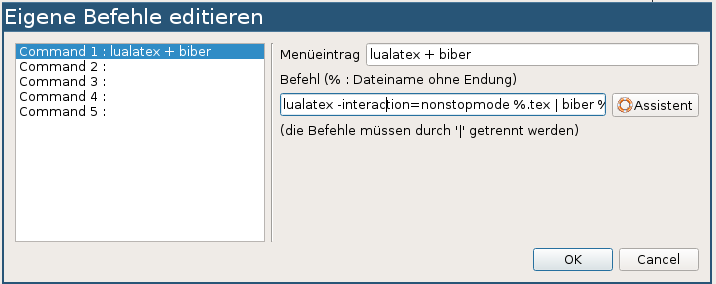
\includegraphics[width=12cm]{Plots/texmaker.png}
    \caption{Screenshot zur Erstellung des Kompilier-Befehls in Texmaker}
    \label{fig:texmaker}
\end{figure}


In Abbildung \ref{fig:texmaker} ist ein Screenshot des Befehlsmenü gezeigt. Ihren Befehl können Sie nun im Drop-Down-Menü zum 
Kompilieren des Dokuments auswählen und mit einem Klick auf den Pfeil starten.

\subsubsection{Aufräumen}

Nach einem \LaTeX-Fehler ist es oft notwendig, die erstellten Hilfsdateien zu löschen.
Klicken Sie hierzu auf \emph{Werkzeuge}→\emph{Aufräumen}.


\section{\LaTeX-Grundlagen}

Bitte beachten Sie beim Schreiben der Arbeit folgende Konventionen bzw. Grundlagen:

\begin{itemize}
    \item \textbf{Abschnitte und Zeilenumbrüche} \\
        Es sollten im Fließtext keine Zeilenumbrüche mit \textbackslash\textbackslash \ erzwungen werden.
        Schreiben Sie höchsten einen Satz in eine Code-Zeile.
        Absätze werden im Code mit einer Leerzeile markiert und dann entsprechend der Einstellung von \texttt{parskip} in der Dokumentenklasse gesetzt.
    \item \textbf{Kursiv/Aufrecht} \\
        \begin{itemize}
            \item Variablen und physikalische Größen werden kursiv gesetzt. 
            \item Einheiten werden immer aufrecht und mit einem halben Leerzeichen Abstand zur Zahl gesetzt. Nutzen Sie \texttt{siunitx}!
            \item Mathematische Konstanten und Funktionen werden ebenfalls aufrecht gesetzt. Zum Beispiel die Eulersche Zahl e, das imaginäre i und das infinitesimale d.
                Im Mathematikmodus können Sie dies mit dem Befehl \verb_\mathrm{}_ erreichen. Für die Funktionen stellt \LaTeX \ Befehle bereit, z.B. \verb+\arccos+.
            \item Integrand und ein $\mathrm{d}x$ sollten ebenfalls durch ein kleines Leerzeichen (\verb+\,+) getrennt werden.
        \end{itemize}
        


\end{itemize}

\subsection{Zahlen und Einheiten}

Jede Zahl, jede Einheit und jede Zahl mit Einheit sollte mit Hilfe der in dem Paket \texttt{siunitx} zur Verfügung gestellten Befehle gesetzt werden.
Grundsätzlich gilt: Einheiten werden aufrecht gesetzt und haben ein kleines Leerzeichen (\verb+\,+) Abstand zu ihrer Zahl. 
Werden Fließkommazahlen ohne \texttt{siunitx} gesetzt, entsteht ein hässlicher Leerraum zwischen Komma und erster Nachkommastelle, da \LaTeX \ das Komma nicht als Dezimaltrennzeichen, sondern als Satzzeichen interpretiert.

Das Paket wurde mit deutschen Spracheinstellungen (also mit Komma als Dezimaltrennzeichen und $\cdot$ zwischen Zahl und Zehnerpotenz) geladen, sowie mit den Einstellungen, dass die Standardabweichung stets durch $\pm$ abgetrennt wird und Einheiten falls nötig als Brüche ausgegeben werden.

\begin{table}
    \centering
    \caption{Beispiele für siunitx}
    \label{tab:si}
    \begin{tabular}{l r}
        \toprule
        Befehl     &   Ergebnis \\
        \midrule
        \verb+\num{1.2345}+ & \num{1.2345} \\
        \verb+\num{1.2e3}+ & \num{1.2e3} \\
        \verb_\num{1.2 +- 0.2}_ & \num{1.2+-0.2} \\
        \verb+\num{10000}+ & \num{10000} \\
        \verb+\si{\meter\per\second}+ & \si{\meter\per\second} \\
        \verb+\SI{1.2(1)}{\micro\ampere}+ & \SI{1.2(1)}{\micro\ampere} \\
        \verb+\SI{1.2\pm0.1e3}{\kilo\gram\per\cubic\meter}+ & \SI{1.2\pm0.1e3}{\kilo\gram\per\cubic\meter} \\
        \bottomrule 
    \end{tabular}
\end{table}

Das Paket stellt unter anderem die drei wichtigen Befehle
\begin{itemize}
    \item \texttt{\textbackslash num\{Zahl\}},
    \item \texttt{\textbackslash si\{Einheit\}} und
    \item \texttt{\textbackslash SI\{Zahl\}\{Einheit\}}
\end{itemize}
zur Verfügung.
Diese Befehle sollten stets genutzt werden, wenn Zahlen angegeben werden. 
Sie funktionieren sowohl im Text- als auch im Mathematikmodus.
In Tabelle \ref{tab:si} sind einige Beispiele aufgetragen. Bitte lesen Sie die Dokumentation \cite{siunitx}.

\subsection{Das Literaturverzeichnis}

Das Literaturverzeichnis wird mit Hilfe von BibLaTeX und biber erstellt.
Tragen Sie alle ihre Quellen in die Datei \texttt{references.bib} ein, Sie enthält bereits
einige Beispiele. Für weitere Informationen lesen Sie bitte die Dokumentation \cite{biblatex}.

Im Text können Sie mit \verb_\cite{kürzel}_ zitieren. Seitenzahlen geben Sie in eckigen Klammern an:
\verb_\cite[10]{kürzel}_. 

Das Literaturverzeichnis ist so eingestellt, dass es Ihre Quellen in alphabetischer Reihenfolge nach Autoren nummeriert.
Möchten Sie das Literaturverzeichnis nach der Reihenfolge des Auftauchens im Text sortieren, fügen sie die Paktetoption \texttt{sorting=none} beim Laden
des BibLaTeX-Pakets hinzu.

Den Zitier- und Bibliographie-Stil geben sie mit der Option \texttt{style=Stil} an. Die beiden gebräuchlisten Stile sind \texttt{numeric} und \texttt{alphabetic}. 
Bei \texttt{numeric} werden die Quellen durchnummeriert, bei \texttt{alphabetic} wird ein Buchstabenkürzel aus Autor(en)-Name(n) und Jahr verwendet.
Für weitere Stile konsultieren Sie bitte die Dokumentation: \cite{biblatex}.

Ein Beispiel für das Zitieren eines Buches lautet so \cite{handbook_adhesives},
wissenschaftliche Artikel hingegen werden so \cite{einstein} zitiert.

Damit das Literaturverzeichnis erstellt wird, ist ein Aufruf von \texttt{biber} nach einem ersten kompilieren mit \texttt{lualatex} nötig.
Danach muss das Dokument erneut mit \texttt{lualatex} kompiliert werden. 

Zum korrekten Kompilieren des Dokuments siehe Kapitel \ref{make}.

\section{Abbildungen und Tabellen}

\subsection{Abbildungen}

Achten Sie bei ihren Plots auf ausreichend große Achsenbschriftungen, ausreichende Schriftdicken und gut unterscheidbare Farben.
Im Idealfall haben Sie im Plot und der Arbeit die gleiche Schriftgröße und Schriftart.
Dies lässt sich durch Erstellen des Plots in der korrekten Größe und Einbinden mit dem optionalen Argument \texttt{scale=1} erreichen. Ein Beispiel sehen Sie in Abbildung \ref{fig:bsp}.

Nutzen Sie wenn möglich Vektorgrafiken (pdf) und nur in Ausnahmen Rastergrafiken wie .png oder .jpg.
Setzen Sie Punkte hinter Abbildungsunterschriften.

\begin{figure}
    \centering
    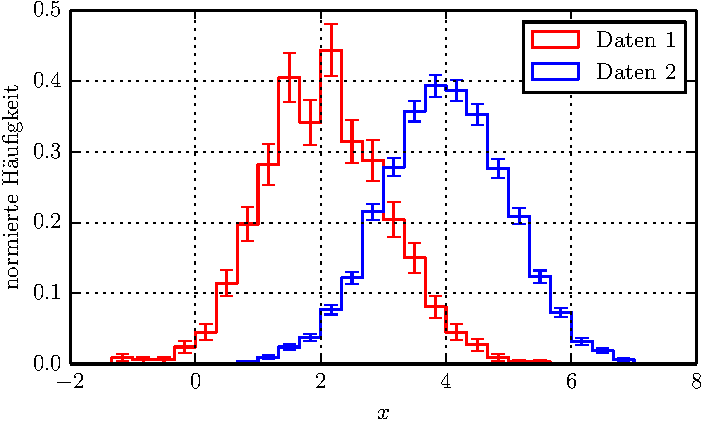
\includegraphics[scale=1]{./Plots/Histogramm.pdf}
    \caption{Ein Histogramm mit Fehlerbalken für zwei Datensätze, Schriftgröße und -art entsprechen der des Dokuments.}
    \label{fig:bsp}
\end{figure}

\subsection{Tabellen}

Tabellen sollten so einfach wie möglich aufgebaut sein, verzichten Sie auf zu viele Linien. In fast allen Fällen reichen drei horizontale Linien aus, jeweils über und unter der Tabelle und zwischen den Spaltenüberschriften und der eigentlichen Tabelle.

Das Paket \texttt{booktabs} stellt hierfür \verb_\toprule_, \verb_\midrule_ und 
\verb_\bottomrule_ zur Verfügung.
Das Paket \texttt{siunitx} stellt eine extrem mächtige neue Spalteneinstellung bereit: \texttt{S}, mit ihr können Zahlen und Einheiten sehr sauber und gut ausgerichtet gesetzt werden.

Diese Vorlage geht von Tabellenüberschriften aus, möchten Sie dagegen Tabellenunterschriften entfernen Sie das entsprechende optionale Argument für die Dokumentenklasse in der Präambel.

Ein Beispiel ist Tabelle~\ref{tab:bsp}.
\begin{table}
    \centering
    \caption{Beispieltabelle mit willkürlichen Werten, für die Zahlenwerte wurde die S-Option aus \texttt{siunitx} verwendet.}
    \label{tab:bsp}
    \begin{tabular}{S[table-format=4.2] S[table-format=3.2]}
        \toprule
        {$p \mathrel{/} \si{\pascal}$}  & {$T \mathrel{/} \si{\kelvin}$} \\
        \midrule
        1024,23 & 273,15 \\
        1025,31 & 274,5 \\
        1026,27 & 276,2 \\
        \bottomrule
    \end{tabular}
\end{table}


\appendix
% Hier beginnt der Anhang, nummeriert in lateinischen Buchstaben
\section{Ein Anhangskapitel}

Hier könnte ein Anhang stehen, falls Sie z.\,B.\ Code, Konstruktionszeichnungen oder Ähnliches mit in die Arbeit bringen wollen.
Im Normalfall stehen jedoch alle Ihre Resultate im Hauptteil der Bachelorarbeit und ein Anhang ist überflüssig.


%\backmatter
\printbibliography

\cleardoublepage
% From https://www.tu-dortmund.de/studierende/im-studium/pruefungsangelegenheiten/allgemeine-vordrucke/
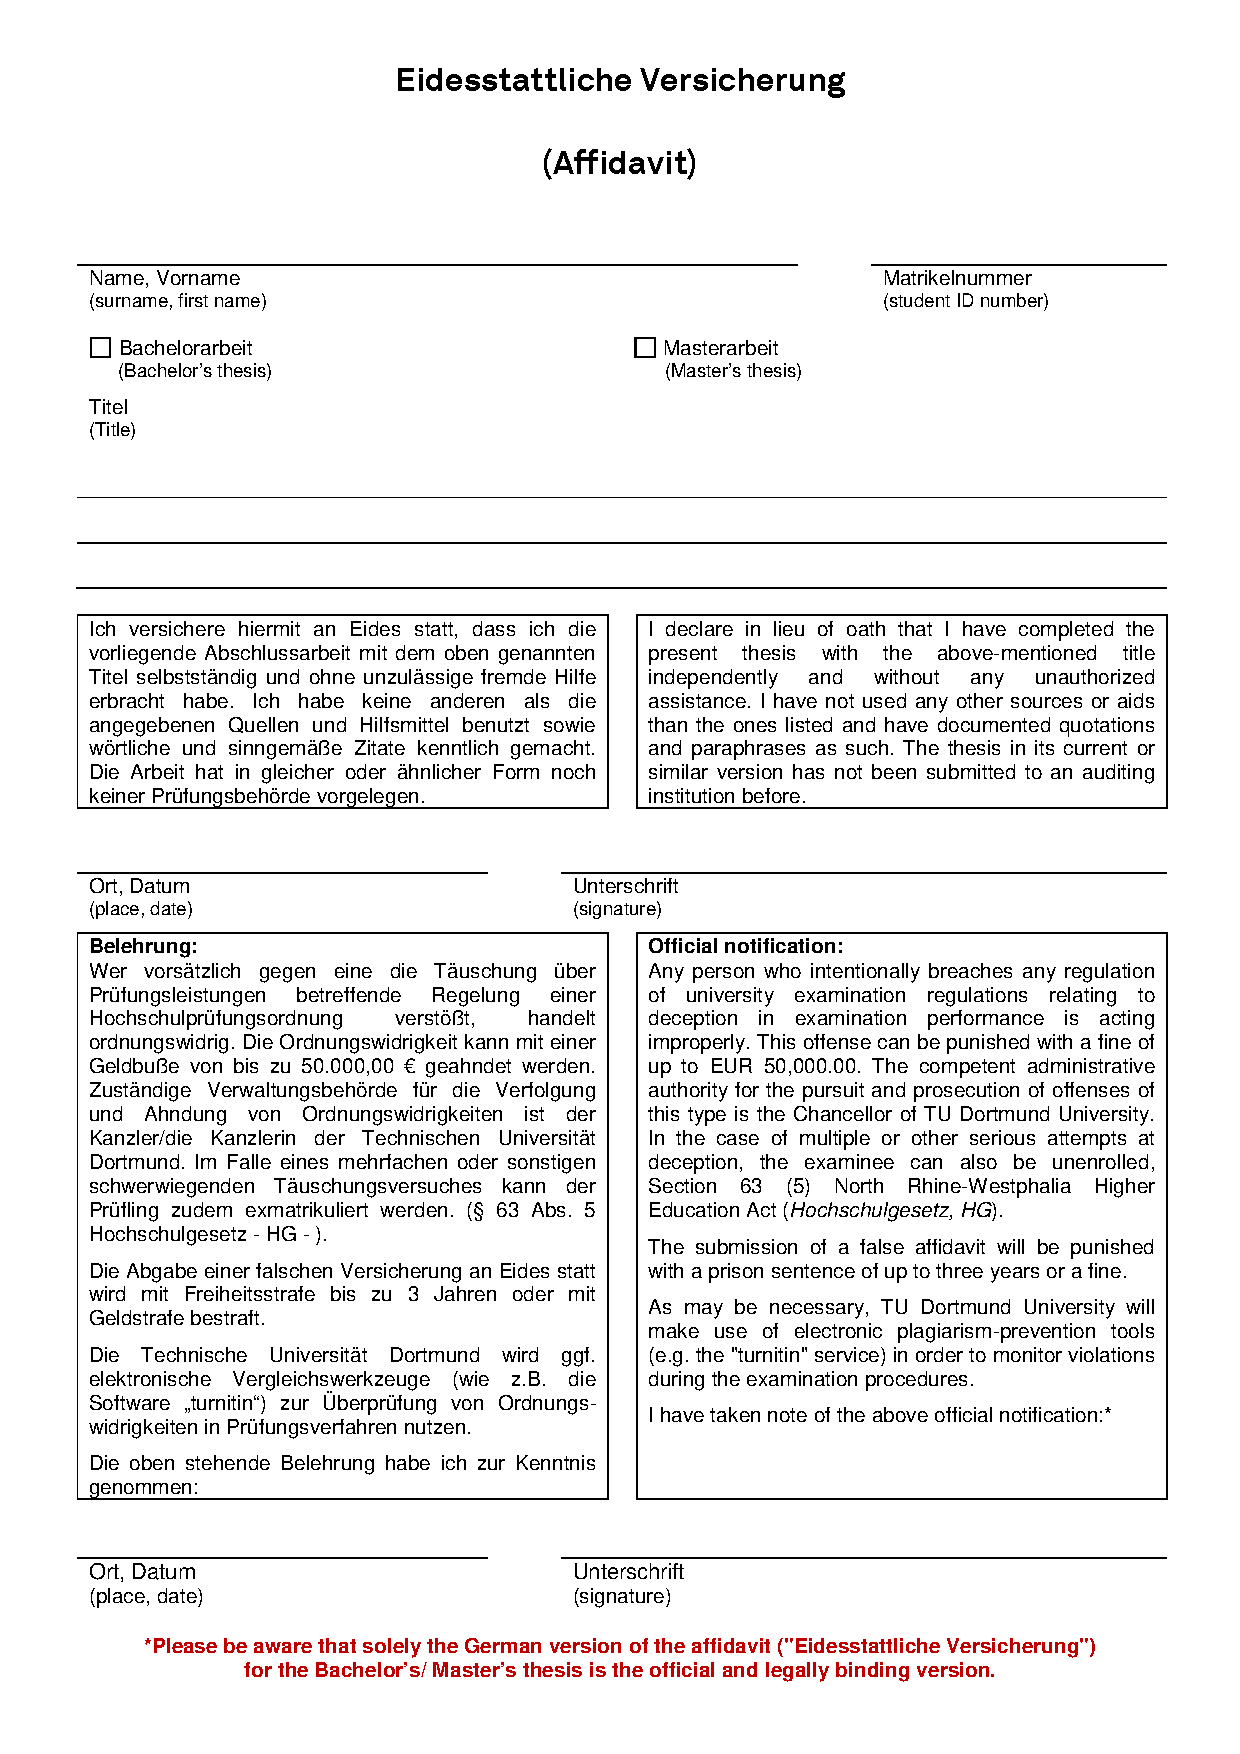
\includepdf{content/Eidesstattliche_Versicherung.pdf}

\end{document}
